\chapter{Technical Documentation}
\label{chapter:technical_documentation}

\section{Attachments}

This thesis is accompanied with a number of file attachments. These files include the C++ source code of the algorithms described in this thesis, several Python scripts which were used to identify the parameters of the servo and motor models, and code for integration with \gls{ROS} and with the hardware of the experimental RC vehicle and with the F1/10 Gazebo simulator. The files are organized in the following directory structure:

\vspace{0.25cm}
\dirtree{%
	.1 /.
	.2 arduino\DTcomment{C code for two Arduino microcontrollers}.
	.3 steering\_node.
	.3 motor\_shaft\_encoder.
	.2 \textbf{catkin\_ws}\DTcomment{ROS Catkin workspace of the Racer project}.
	.3 \textbf{src}.
	.4 \textbf{racer}\DTcomment{our main ROS package}.
	.5 circuits\DTcomment{circuit definiton files (YAML)}.
	.5 \textbf{include}.
	.6 \textbf{racer}\DTcomment{C++ code under the \texttt{racer} namespace}.
	.6 racer\_ros\DTcomment{code for integration with ROS (C++)}.
	.5 launch\DTcomment{custom launch files}.
	.5 maps\DTcomment{maps recorded using SLAM (YAML+PGM)}.
	.5 scripts\DTcomment{ROS nodes for debugging and telemetry (Python)}.
	.5 src\DTcomment{ROS nodes for the racing agent (C++)}.
	.4 racer\_msgs\DTcomment{custom ROS messages}.
	.4 racer\_sensors\DTcomment{sensor adjustments and odometry}.
	.4 racer\_simulator\DTcomment{integration with the F1tenth simulator}.
	.5 launch\DTcomment{launch and Rviz configuration files}.
	.5 src\DTcomment{ROS nodes for integration with the simulator (Python)}.
	.2 \textbf{experiments}.
	.3 \textbf{algorithm\_testing}\DTcomment{testing the algorithms outside of ROS (C++)}.
	.3 model\_fitting\DTcomment{identification of actuator models (Python)}.
	.4 motor\_rpm.
	.4 servo\_pwm\_to\_steering\_angle.
	.4 servo\_setting\_time.
	.2 media.
	.3 experimental\_vehicle\_gym\DTcomment{Videos of the self-driving RC car}.
	.3 simulator\DTcomment{Screenshots from Rviz and Gazebo}.
}
\vspace{0.5cm}

In rest of this chapter, we will go over the different parts of the project and explain how to use them and how to work with them. We will first describe how to use the ``standalone'' experiments in the \texttt{experiments} directory and later we describe the ROS project located in the \texttt{catkin\_ws} directory and we go over the steps necessary to build and run the project in the simulator and on custom hardware. Finally, we will describe the ideas behind the C++ code of the algorithms located in the \texttt{catkin\_ws/src/racer/include/racer} directory.

\section{Track Analysis and Trajectory Planning}

In order to test the track analysis algorithm from Section~\ref{sec:track_segmentation} and the \gls{SEHS} and Hybrid A* trajectory planning algorithms described in Chapter~\ref{chapter:trajectory_planning}, we wrote two C++ programs to test these algorithms on different inputs and to visualize their outcomes.

\subsection{Requirements and Compilation}

In order to compile and run these test programs, we recommend using a PC running a Linux distribution. Both programs were also successfully tested on Microsoft Windows 10 with \textit{Windows Subsystem for Linux} (WSL) 2 and the \textit{X Window System}, such as \textit{Xming X Server}\footnote{\url{http://www.straightrunning.com/XmingNotes/}}, installed. The programs are written using C++17 and they are meant to be compiled using the G++ 9.2 compiler\footnote{\url{https://gcc.gnu.org/gcc-9/}}.

To visualize the outputs of the algorithms, we use the \textit{Matplotib} library and its C++ binding library \texttt{matplotlib-cpp}. The source code of this library is available in a public Git repository under the MIT licence hosted on GitHub\footnote{To see the code of the libraryt at the time of writing, see \url{https://github.com/lava/matplotlib-cpp/tree/d612b524e10ebdd43d3a8889a95e84c017ad65af}. Our code might not be compatible with newer revisions of the library.}. In order to set up this library, install the dependencies of the library first\footnote{The instructions are available at \url{https://github.com/lava/matplotlib-cpp/tree/d612b524e10ebdd43d3a8889a95e84c017ad65af#installation}.} and then clone the repository using \texttt{git}\footnote{\url{https://git-scm.com/}} and change the repository to the version needed in our code:

\begin{verbatim}
 > cd /experiments/algorithm-testing/include
 > git clone https://github.com/lava/matplotlib-cpp
 > cd matplotlib-cpp
 > git checkout d612b524e10ebdd43d3a8889a95e84c017ad65af
\end{verbatim}

To compile and link the source code into executable binaries, use the prepared \texttt{Makefile}:

\begin{verbatim}
 > cd /experiments/algorithm-testing
 > make
\end{verbatim}

This script will create a new subdirectory \texttt{bin} and place the newly created binaries in there.

The C++ code includes header files from the \texttt{catkin\_ws/src/racer/include} directory. If you make adjustments to the directory structure, compilation might fail because \texttt{g++} will not be able to find the included files. In such case, edit the \texttt{Makefile} and fix the paths of the \texttt{-I} options to match your directory structure.

\subsection{Usage}

\paragraph{Track Analysis}

The track analysis algorithm is easy to test for a circuit:

\begin{verbatim}
 > ./bin/track_analysis <circuit-definition-file>
\end{verbatim}

The program will output the time each of the steps of the analysis takes and finally it will open a window with the map of the circuit and with marked corners which were detected.

\paragraph{Trajectory Planning}
To test the trajectory planning algorithm, run this command:

\begin{verbatim}
 > cd /experiments/algorithm-testing
 > ./bin/planning_benchmark <n> <timeout> <circ-1> <circ-2>...
\end{verbatim}

The parameter \texttt{<n>} determines how many times each algorithm with a given set of parameters for a given circuit will be run in order to calculate the average search time. The parameter \texttt{<timeout>} determines the time limit for a single search in milliseconds. At least one path to a circuit definition file has to be provided, but the binary accepts multiple of them and it will loop over all of them and execute the search for each of them with all of the combinations of the parameters.

The program tests both Hybrid A* and the \gls*{SEHS} algorithms with several different combinations of discretization parameters. The output of the program will be a comma separated values file with the summaries of each test. After each algorithm is tested with each different set of parameters, the found trajectory and the speed profile is shown in a pop-up window.

\subsection{Circuit Definition File Format}

Each circuit is defined with a simple text file with the following structure:

\begin{verbatim}
 <pgm-file>
 <occupancy-grid-resolution>
 <ix> <iy> <itheta>
 <c1x> <c1y>
 <c2x> <c2y>
\end{verbatim}

The first line contains the path to the occupancy grid file relative to the circuit definition file. The second line contains a decimal number specifying the resolution of the occupancy grid in meters (typical value is \num{0.05}). The third value describes the initial position and orientation of the vehicle. The rest of the file form lines of $x$ and $y$ coordinates of checkpoints along the circuit. At least two checkpoints are expected, but there is no hard upper limit. Examples of circuits can be found in the \texttt{/experiments/\-algorithm\-\_testing/\-test-inputs} directory.

\paragraph{PGM File Format Limitations}

The occupancy grid is loaded from a bitmap stored in a PGM file format\footnote{\url{http://netpbm.sourceforge.net/doc/pgm.html}}. We support only the \textit{Plain PGM format} with the magic number \texttt{P2} and the pixels represented by ASCII encoded decimal numbers. The numbers must be between \num{0} and \num{127}. Some bitmap editors, such as GIMP, produce images with pixel values outside of this range, and these files need to be edited manually before they can be supplied to the test programs.

\section{Actuator Models}

This section describes the scripts we wrote in order to fit the parameters of the actuator models as described in Section~\ref{sec:actuators_model}.

\subsection{Requirements}

In order to open and run the actuator model fitting scripts, you need to install Python 3.6\footnote{\url{https://www.python.org/}} and the Jupyter Notebook\footnote{\url{https://jupyter.org/}}. The scripts also need the following Python libraries installed on your computer:

\begin{itemize}
	\item Matplotlib\footnote{\url{https://matplotlib.org/}}
	\item Pandas\footnote{\url{https://pandas.pydata.org/}}
	\item Numpy\footnote{\url{https://numpy.org/}}
	\item SciPy\footnote{\url{https://www.scipy.org/}}
\end{itemize}

\subsection{Usage}

To open the scripts, start the Jupyter notebook:

\begin{verbatim}
 > cd /experiments/model_fitting
 > jupyter notebook
\end{verbatim}

Your browser should open with the Jupyter interface. From here, you can open one of the three subdirectories with the experiments: \texttt{motor\_rpm}, \texttt{servo\_pwm\-\_to\_\-steering\_angle}, and \texttt{servo\_setting\_time}. Each directory contains a \texttt{.ipynb} script which you can view and re-run and the data with the measurements.

\section{ROS Project}

\gls{ROS} is an open-source set of libraries and tools built on top of Linux. Processes running under this operating system are referred to as nodes and they can be distributed across multiple computers connected over a wired or wireless network or through a serial port. Nodes can be programmed in many different programming languages but the most common and officially supported languages are Python and C++.

Nodes communicate between each other using a publisher/subscriber pattern. A node can advertise any number of topics through which it publishes its outputs in a form of messages. It can also subscribe to topics advertised by other nodes and it can work with the received messages as its outputs. This way it is possible to create a complex system by combining many small and simple specialized nodes.

Each topic has an assigned message type which defines the structure of the data. There is a large number of standard messages which are used by authors of public libraries. This way it is often possible to replace one library with a different one without additional changes to other nodes. This can be useful for example when one sensor is replaced by a device of the same type but from a different vendor whose \gls*{ROS} node publishes the same standard message type. Programmers can also define their custom message types which are better suited for their application.

\gls*{ROS} comes with a variety of tools for debugging and visualization of the data passed through the topics. One of these tools is \verb|Rviz|. It is a convenient way of visualizing the current state of the system. We use this tool to visualize the telemetry data from the vehicle on a laptop while it is driving along the racing circuit.

We use the latest stable release of \gls*{ROS} at the time of writing this thesis named ``Melodic Morenia'' which is compatible with Ubuntu 18.04 LTS. All the installation instructions assume that the user is running this version of Ubuntu as their operating system. Further information about \gls*{ROS} and tutorials which describe how to work with it are available on the official website of the \gls*{ROS} project\footnote{\url{https://www.ros.org}}.

\subsection{Architecture of the Distributed System}

The setup of our robot consists of the NVIDIA Jetson Nano board which is mounted on the vehicle, two Arduinos which are connected to the Jetson through a serial port, and a notebook which is connected to Jetson over Wi-Fi. Jetson acts as a \gls*{ROS} master machine, Arduinos act as an interface between Jetson and low-level hardware, and the notebook is used only to monitor telemetry data. The graph of this architecture and the connected sensors is depicted in Figure~\ref{fig:ros_diagram}.

\begin{figure}
	\centering
	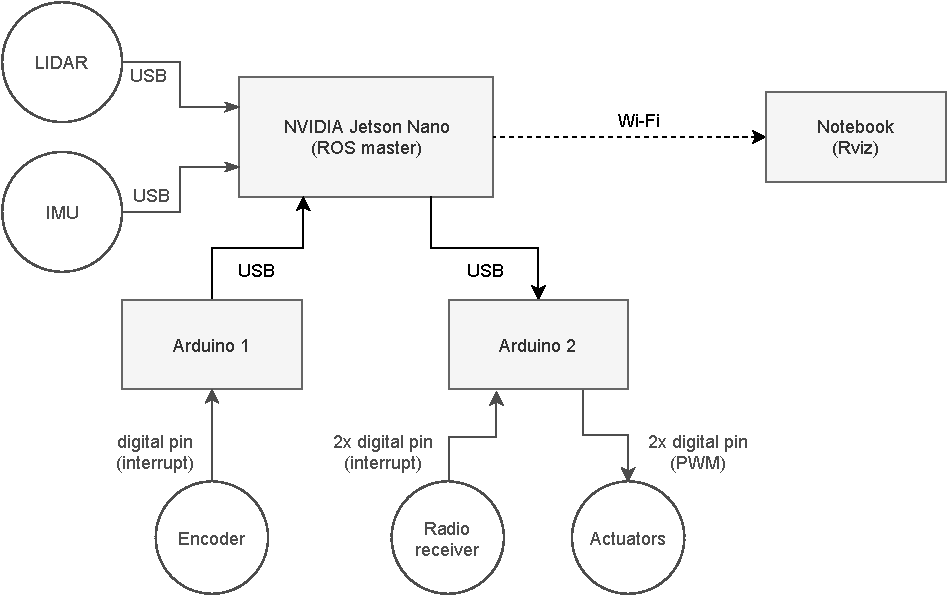
\includegraphics[width=125mm]{../img/ros_diagram}
	\caption{This figure shows how the computers and sensors which make up the experimental vehicle are connected with each other and the direction of data flow between the devices.}
	\label{fig:ros_diagram}
\end{figure}

The communication between the Arduinos and the Jetson takes place over USB. This is possible thanks to the \verb|rosserial| package\footnote{\url{http://wiki.ros.org/rosserial}}. The Arduinos need to include the \verb|ros_lib| library which allows it to subscribe to topics and to publish messages. On Jetson, the communication on each serial port is handled by an instance of a \verb|rosserial_python| node.

\subsubsection{Coordinate Frames}

\Gls{ROS} includes a very useful way of keeping track of the relative position between different parts of the robot and the position of the robot itself on a map. The package which provides this functionality is called \verb|tf|\footnote{\url{http://wiki.ros.org/tf}}. \verb|tf| maintains a tree structure of coordinate frames and it keeps track of transformations between these coordinate frames as they change over time. The updates to the transformations are shared through a regular \gls*{ROS} topic called \verb|tf| of the \texttt{tf/tfMessage}\footnote{\url{http://docs.ros.org/kinetic/api/tf/html/msg/tfMessage.html}} type. The \verb|tf| package provides libraries for both Python and C++ which make accessing the current state of the whole system and manipulating with the linear transformations easy.

Our implementation adheres to the standard naming convention of coordinate frames as it is defined in \gls{REP} 105\footnote{\url{https://www.ros.org/reps/rep-0105.html}}. The vehicle has a \verb|base_link| frame attached to it. Each of the sensors has their own coordinate frame and there is a static transformation between the sensor and the base link using the \texttt{static\_\allowbreak transform\_\allowbreak publisher} node from the \verb|tf| package. The \gls*{IMU} gives us the current roll and pitch of the vehicle. We use the \texttt{hector\_imu\_attitude\_tf} node\footnote{\url{https://github.com/tu-darmstadt-ros-pkg/hector\_slam/tree/catkin}} to publish this transformation between \texttt{base\_link} and \texttt{base\_footprint}, which is the ``stabilized'' coordinate frame. The root (``fixed'') \verb|tf| frame is called \verb|map|. The transformation between the \verb|map| frame and the \verb|base_footprint| represents the pose of the vehicle on the map. This transformation is calculated and published through different nodes in the mapping and racing tasks and we will come back to it later.

\subsubsection{Sensors}
\label{sec:sensors}

Each of the sensors connected through USB uses their own drivers for communication over the serial link. Luckily, open-source \gls*{ROS} packages for both the \gls*{LIDAR} and the \gls*{IMU} are available and both of them publish the data in the form of standard \verb|sensor_msgs/LaserScan|\footnote{\url{http://docs.ros.org/melodic/api/sensor\_msgs/html/msg/LaserScan.html}} and \verb|sensor_msgs/Imu|\footnote{\url{http://docs.ros.org/melodic/api/sensor\_msgs/html/msg/Imu.html}} messages.

The data from the motor shaft encoder is published as a \verb|std_msgs/Float64| message and it contains the number of revolutions since the Arduino was last powered or reset.

The raw data we receive from the \gls*{LIDAR} and the \gls*{IMU} are not readily usable. We had to introduce a layer of preprocessing for both these sensors:

\begin{enumerate}
	\item The coordinate frame of the \gls*{IMU} is not aligned with the coordinate frame of the vehicle. Even though it should be possible, we were not able to get correct roll and pitch transformations using the \texttt{static\_transform\_\-publisher} node of the \texttt{tf} package. To overcome this issue, we implemented a custom node in C++ called \texttt{fix\_imu} in the \texttt{racer\_sensors} package, which publishes the correct transformation. We also set positive values on the diagonals of covariance matrices to make the \gls*{IMU} message valid, because the \gls*{ROS} package for the \gls*{IMU} we use  \verb|bno055_usb_stick|\footnote{\url{https://github.com/yoshito-n-students/bno055\_usb\_stick}} does not set them correctly. The configuration for the \gls*{IMU} is stored in \texttt{/catkin\_ws/\allowbreak src/\allowbreak racer/\allowbreak launch/\allowbreak imu.launch}.

	\item The \gls*{LIDAR} is rigidly attached to the vehicle and so the laser scan is affected by the roll and pitch of the vehicle. We use \texttt{LaserScanBoxFilter} from the \texttt{laser\_filters} package\footnote{\url{http://wiki.ros.org/laser\_filters}} to remove points which are too close to the ground (the vehicle might see the ground when it is slowing down or braking) and which are too high above the ideal plane (the vehicle might see the ceiling or over the obstacles when it accelerates). The configuration for the \gls*{LIDAR} is stored in \texttt{/catkin\_ws/\allowbreak src/\allowbreak racer/\allowbreak launch/ydlidar.launch}.
\end{enumerate}

\subsection{Mapping}

In order to race, our vehicle needs a map of the racing track. The robot can create its own map using an algorithm called \gls{SLAM}. We use a library called Hector \gls*{SLAM} created by a team from the Technical University of Darmstadt.

To make things simple, we steer the vehicle manually using its remote controller. The robot collects data from the \gls*{LIDAR} as it moves along the track and it performs scan matching between the \gls*{LIDAR} scans and a 2D occupancy grid which it has built so far. For an already built part of the map and a \gls*{LIDAR} scan consisting of $n$ points, the task of the scan matching algorithm is to find a rigid body transformation $\xi =\left( p_x, p_y, \phi\right)$, which gives best alignment with the already built map. The authors formulate this problem as an optimization problem for solving in \cite{HectorSlam}:

$$
\xi^* = \underset{\xi}{\arg\min} \sum_{i=1}^n\left[ 1 - M\left( S_i\left( \xi\right)\right)\right]^2,
$$

where $S_i\left(\xi\right)$ are the world coordinates of scan point $s_i$ after applying the transform $\xi$ and the function $M$ gives the value of the occupancy grid at the given coordinates. After obtaining the transformation, the laser scan is aligned with the occupancy grid and each endpoint of a laser ray is marked as an obstacle into the occupancy grid.

Hector SLAM provides a \gls*{ROS} node \verb|hector_mapping| which subscribes to a topic providing \verb|sensor_msgs/LaserScan| messages and publishes its output in a topic of type \verb|nav_msgs/OccupancyGrid|\footnote{\url{http://docs.ros.org/melodic/api/nav\_msgs/html/msg/OccupancyGrid.html}}. The node also publishes a \verb|tf| transformation between the \verb|map| frame and the \verb|base_footprint| frame. An important parameter is the resolution of the occupancy grid which we chose to be \SI{5}{\centi\meter}. When the mapping is complete, the final map can be saved into a file using a \verb|map_saver| node from the \verb|map_server| package\footnote{\url{http://wiki.ros.org/map\_server\#map\_saver}}. We prepared a \gls*{ROS} launch file with the configuration of all nodes necessary for this task. This configuration is included in the attached files in \texttt{/catkin\_ws/\allowbreak  src/\allowbreak  racer/\allowbreak  launch/create\_map.launch}.

\subsection{Racing}

Racing is the most important and the most complicated part of the implementation. It can be split into three groups of \gls*{ROS} nodes: odometry and localization, agent behavior, and the hardware interface.

\subsubsection{Map}

We use \verb|map_server| node of the \verb|map_server| package to serve the previously recorded occupancy grid to the other nodes. The map is stored in two files: a \verb|.yaml| file with map metadata and a \verb|.pgm| file with the occupancy grid stored as a bitmap. It is necessary that the \verb|.yaml| configuration file contains a correct relative path to the bitmap file. The map server publishes a topic called \verb|map| of type \verb|nav_msgs/OccupancyGrid|. This node also provides a service for one-time retrieving the map without subscribing to the topic.

\paragraph{Costmap} In order to prevent collisions, we use a \gls*{ROS} package \verb|costmap_2d|\footnote{\url{http://wiki.ros.org/costmap\_2d}} to inflate the areas around obstacles according to a bounding rectangle around the vehicle. The result of this node is another \verb|nav_msgs/OccupancyGrid| topic with cell values marking the ``cost'' of each cell instead of the regular ternary status (free/obstacle/unknown). The higher the cell cost is, the closer the cell is to an obstacle. Values above certain threshold value are considered ``lethal'' and if the center of the vehicle were in this position it would be colliding with an obstacle. Collision detection is then just a matter of a single query into the occupancy grid to check if the cell which contains the center point of the vehicle.

This \verb|costmap_2d| can also work directly with the laser scan from the \gls*{LIDAR} and overlay it with the map using the latest \verb|tf| transformation between the \verb|map| and \verb|lidar| coordinate frames and mark obstacles which were not present during mapping into the resulting occupancy grid. Unfortunately, this feature was flaky and we had to disable it in the final version of our configuration when we tested it on the RC car. The laser frame would often be misaligned with the original map for a brief moment and it would mark certain areas of free space as obstacles. The ``clearing'' feature, which is supposed to remove obstacles from the costmap based on new laser scans, did not work properly and the map soon became filled with ghost obstacles. When we tested this package in the simulator, it yielded better results, but we still observed many ghost obstacles.

\subsubsection{Odometry and Localization}

Odometry is an estimate of how position of the robot changes over time based on data from sensors which measure the movement of the robot. Odometry is supposed to be continuous and there should not be any sudden changes in the position of the vehicle.

Our vehicle has two sources of odometry: the number of revolutions of the motor shaft and the accelerations measured by the IMU. We implemented a simple \gls*{ROS} node called \verb|odometry_node| in C++ which subscribes to the motor shaft encoder and the steering commands supplied to the vehicle. From the number of revolutions and an assumption that the wheels are not skidding we can estimate the distance the vehicle travelled since the last update. From the steering command, we can estimate the steering angle of the front wheels of the vehicle. From these two inputs, we can estimate how the vehicle body translated and rotated using a simple kinematic vehicle model. This approach was inspired by the MIT RACECAR VESC odometry \gls*{ROS} node\footnote{\url{https://github.com/mit-racecar/vesc}}. Source code of the odometry node is located in the attachments in \texttt{/catkin\_ws/src/racer\_sensors}.

The data from the odometry node and the \gls*{IMU} are then fused into a single estimate using the \verb|ekf_localization_node| node from the \texttt{robot\_localization} package\footnote{\url{http://docs.ros.org/melodic/api/robot\_localization/html/index.html}}. This node uses \gls*{EKF} to estimate the most likely location from the input sources and their covariances. This node produces a \verb|tf| transform between the \verb|odom| and \verb|base_footprint| frames. We also tried to use the \gls*{ROS} package \texttt{robot\_pose\_ekf} which also implements an \gls*{EKF}, but the results were less accurate.

The data from the odometry sensors is inherently noisy and inaccurate and the estimated position of the robot will become more and more inaccurate over time. This phenomenon is referred to as drift. To counteract the drift, we perform a correction using the \gls*{AMCL} algorithm. This algorithm uses the data from the \gls*{LIDAR} to determine the position of the vehicle in the map based on the distances to the obstacles around it. Unlike odometry, the sequence of position updates is not expected to be continuous and the resulting location can in theory be a point anywhere on the map. We use an implementation of this algorithm in the \verb|amcl| \gls*{ROS} package\footnote{\url{http://wiki.ros.org/amcl}}. The \verb|amcl| node from this package publishes a \verb|tf| transformation between \verb|map| and \verb|odom| to correct the odometry drift. The \verb|tf| tree is captured in Figure~\ref{fig:tf_tree_racing}.

\begin{figure}
	\centering
	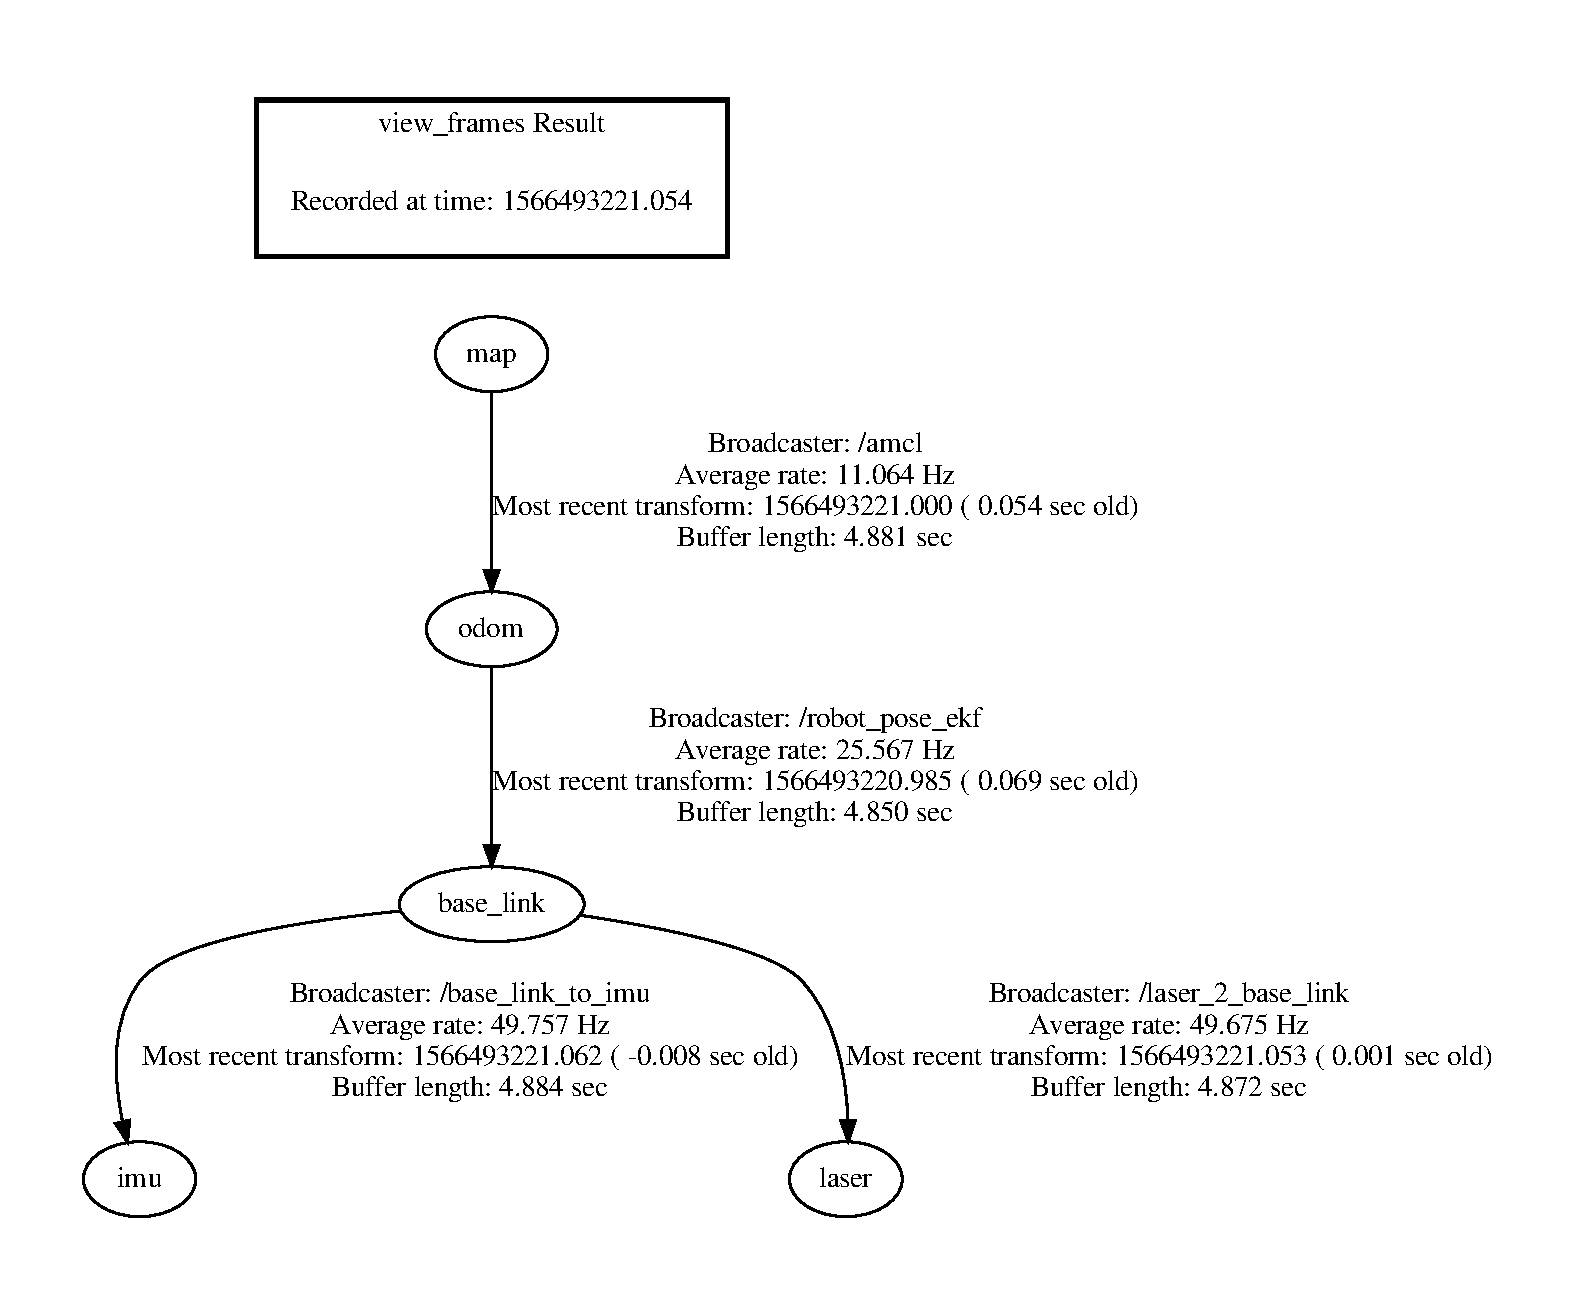
\includegraphics[width=125mm]{../img/racing_tf_tree.pdf}
	\caption{The tree shows which nodes publish transformations between the coordinate frames and at what average rate the transformations are updated. This diagram is the output of the \texttt{view\_frames} diagnostics tool from the \texttt{tf} package.}
	\label{fig:tf_tree_racing}
\end{figure}

Tuning odometry and localization ROS libraries to obtain reliable data at high rates proved to be difficult. In some scenarios, the robot would ``get lost'' when the localization algorithm would match the scan incorrectly and it would report incorrect location of the robot on the map. This can easily lead into a crash of the robot with a wall or an obstacle. The \gls*{AMCL} algorithm will sometimes manage to find the correct location after a few seconds, but in these cases it was necessary to take over control over the vehicle manually with a remote control and stop the vehicle until the robot corrects its location. The \gls*{AMCL} \gls*{ROS} node has many parameters which we spend many hours tuning them in order to get the best possible results. The final configuration is available in \newline\verb|/catkin_ws/src/racer/launch/amcl_localization.launch|.

\subsubsection{Agent Behavior}
\label{sec:agent_impl}

We implemented the individual components of the behavior of the agent, as it was described in Chapter~\ref{chapter:agent} and visualized in Figure~\ref{fig:racing_agent_diagram}, with four \gls*{ROS} nodes as part of the \verb|racer| package we implemented:

\begin{enumerate}
	\item \verb|current_state_node|,	
	\item \verb|circuit_node|,
	\item \verb|planning_node|,	
	\item \verb|dwa_planning_node|.
\end{enumerate}

The C++17 implementation of the \verb|racer| package is located in \texttt{/catkin\_ws/\-src/racer/} and it contains the source code of the individual \gls*{ROS} nodes as well as the source code of the algorithms which were described in this thesis. The definitions of the messages are located in a separate package \texttt{/catkin\_ws/\allowbreak src/racer\_msgs/}. All of the coordinates used by \verb|racer| package nodes are in the global \verb|map| coordinate frame unless stated otherwise.

\paragraph{Current State Node}

This node listens to the \verb|tf| transformations and converts them into a custom message format \verb|racer_msgs/State|. This message contains the 2D position of the vehicle, its orientation, and its immediate speed in the heading direction in the \verb|map| \verb|tf| coordinate frame.

To achieve the highest possible update rate, we had to manually combine the latest odometry estimate \verb|odom -> base_link| and the latest odometry drift correction \verb|map -> odom| by multiplying their transformation matrices. When we tried obtaining the transformation \verb|map -> base_link| from the \verb|tf| library directly, the update rate was the same as the transform published by \gls*{AMCL}. By manually combining the transformations, we would be able to publish the current state estimate in sync with odometry updates.

If we assume that the fused odometry gives us reasonable movement estimates over short time periods and that we use a very recent drift correction, this workaround is reasonable. The maximum rate at which we can control the actuators is \SI{50}{\hertz} and we are able to achieve vehicle state updates at the rate of \SI{25}{\hertz} (see Figure~\ref{fig:tf_tree_racing}).

\paragraph{Circuit Node}

The circuit node analyzes the occupancy grid of the current track based on a circuit definition for the track at the start of the race using Algorithm~\ref{alg:find_pivots}. The circuit definition is a list of checkpoints on the map. The vehicle is supposed to drive along the track in a way such that it passes these checkpoints in the given order. The starting position is considered to be an implicit checkpoint. This list is loaded from a \verb|.yaml| configuration file which contains an array of 2D~point coordinates under the key \verb|check_points|. The coordinates are strings with the $x$ and $y$ coordinate separated by a whitespace. An example of such configuration file with two checkpoints follows:

\begin{verbatim}
check_points:
  - "6.385 -0.521"
  - "-0.639 -4.226"
\end{verbatim} 

Later during the race, this node monitors the state of the vehicle and it produces a list of the next waypoitns in a custom message format
\texttt{racer\_msgs/\allowbreak Waypoints}. The number of waypoints which are published can be configured using the \texttt{lookahead} parameter of the node.

\paragraph{Planning Node}

The planning node plans a trajectory based on the last known state of the vehicle through the next several waypoints directly ahead of the vehicle and publishes it in the form of a custom message type \texttt{racer\_msgs/\-Trajectory}. The planning node uses either the \gls*{SEHS} or the Hybrid A* algorithm based on an parameter passed from a \gls*{ROS} launch file.

\subsubsection{Following Node}

This node listens to the current vehicle state and the planned trajectory topics and it selects the actions for the vehicle using either the \gls{DWA} or the Pure Pursuit algorithms. The strategy which the node uses can be changed via a parameter. The node publishes the actions in two standard message types on two topics. These message types are \verb|geometry_msgs/Twist|\footnote{\url{http://docs.ros.org/melodic/api/geometry\_msgs/html/msg/Twist.html}} and \texttt{ackermann\_msgs/\-AckermannDrive}\footnote{\url{http://docs.ros.org/jade/api/ackermann_msgs/html/msg/AckermannDrive.html}}.. The \texttt{Twist} message type mimics the output of the open source \verb|move_base| \gls*{ROS} package\footnote{\url{http://wiki.ros.org/move\_base}}. The throttle level is stored in the \verb|linear.x| component ant the steering level is stored in \verb|angular.z|. This message is later translated into a \gls*{PWM} signal for the actuators by the hardware interface component. The \texttt{AckermannDrive} message type is necessary to control the vehicle in the simulator.

\subsubsection{Hardware Interface}
\label{sec:hardware-interface}

The \verb|Arduino 2| from Figure~\ref{fig:ros_diagram} has two responsibilities:

\begin{enumerate}[label=(\roman*)]
	\item subscribe to the commands produced by the agent and transform them into electrical signals for the servo and the \gls*{DC} motor,
	\item monitor the input from the radio controller and in case that there is a strong signal, disable the autonomous mode and forward the signal to the actuators to allow the human supervisor to control the vehicle directly.
\end{enumerate}

\paragraph{Conversion of Commands to PWM}

The agent behavior produces actions in the form of two real numbers between $-1$ and $1$ for the steering angle and for the throttle level. These numbers are mapped to \gls*{PWM} duty cycles which are then passed to the actuators through PWM-capable digital pins of the Arduino.

The mapping for the steering servo is straightforward. The $\interval{-1}{1}$ interval is directly mapped to the interval of $\interval{\SI{1200}{\micro\second}}{\SI{1800}{\micro\second}}$ which are the bounds of the servo of our vehicle. The wheels steer to the leftmost position when the duty cycle is set to \SI{1200}{\micro\second}, at \SI{1500}{\micro\second} the wheels are aligned with the body of the vehicle, and at \SI{1800}{\micro\second} the wheels are in the rightmost position.

The mapping of the signal for the \gls*{DC} motor is a bit more complicated. The range of duty cycles $\interval{\SI{1400}{\micro\second}}{\SI{1600}{\micro\second}}$ does not produce enough torque to set the vehicle into motion. The range of $\interval{\SI{1000}{\micro\second}}{\SI{1400}{\micro\second}}$ corresponds to reversing, where at \SI{1000}{\micro\second} the motor spins the fastest in the reversing direction. The range of $\interval{\SI{1600}{\micro\second}} {\SI{2000}{\micro\second}}$ corresponds to going forward, where at \SI{2000}{\micro\second} duty cycle the motor spins the fastest in the forward direction. The boundary values of \SI{1400}{\micro\second} and \SI{1600}{\micro\second} are not fixed and they vary based on how much is the battery charged. We therefore use the following mapping:

\[
	\begin{dcases}
		\interval{-1}{-0.05} & \rightarrow \interval{\SI{1000}{\micro\second}}{\SI{1400}{\micro\second}} \\
		\interval{-0.05}{0.05} & \rightarrow \SI{1500}{\micro\second} \\
		\interval{0.05}{1} & \rightarrow \interval{\SI{1600}{\micro\second}}{ \SI{2000}{\micro\second}}
	\end{dcases}
\]

The limits can be adjusted for different needs, e.g. the maximum speed can be limited by lowering the maximum duty cycle.

\paragraph{Manual Override}

The two signals from the radio receiver are connected to two interrupt pins of the Arduino. By measuring the time difference between the detection of a raising edge and a falling edge of the signal we can determine the width of the duty input cycle. If one of the two signals falls out of the range of $\interval{\SI{1400}{\micro\second}}{\SI{1600}{\micro\second}}$, we consider it to be the supervisors intervention and we will start forwarding the \gls*{PWM} signal directly to the actuators and we will stop processing the commands from the agent. The autonomous mode can be restored by physically pressing the reset button on the board.

\paragraph{Deployment}

The code of the hardware interface described in Section~\ref{sec:hardware-interface} is located in the \texttt{/arduino/steering\_node} directory. The code for the motor shaft encoder described in Section~\ref{sec:sensors} is located in the \texttt{/arduino/motor\_\-shaft\_encoder} directory. In order to upload the code to an Arduino board, use the Arduino IDE\footnote{\url{https://www.arduino.cc/en/Main/Software}}.

\subsection{Requirements and Compilation}

First, you need to install \gls{ROS} \textit{Melodic Morenia} Desktop-Full Install according to the instructions provided on the official website of the project\footnote{\url{http://wiki.ros.org/melodic/Installation}}. Then, you need to clone the following open-source \gls*{ROS} packages from GitHub into the \texttt{/catkin\_ws/src} directory:

\begin{Verbatim}[fontsize=\small]
 > cd /catkin_ws/src
 > git clone --branch 0.4.0 https://github.com/tu-darmstadt-ros-pkg/hector_slam
 > git clone --branch 1.8.8 https://github.com/ros-perception/laser_filters
 > git clone --branch 2.6.5 https://github.com/cra-ros-pkg/robot_localization
\end{Verbatim}

Depending on the \gls*{LIDAR} and the \gls*{IMU} you use, add the corresponding ROS packages. In the case of the sensors described in Appendix~\ref{chapter:hardware}, we installed the following packages:

\begin{Verbatim}[fontsize=\small]
 > cd /catkin_ws/src
 > git clone --branch 1.4.1 https://github.com/YDLIDAR/ydlidar_ros
 > git clone https://github.com/yoshito-n-students/bno055_usb_stick
 > git clone https://github.com/yoshito-n-students/bno055_usb_stick_msgs
\end{Verbatim}

Further, our project depends on these packages, which are part of the full installation of ROS:

\begin{itemize}
	\item \texttt{amcl}\footnote{\url{http://wiki.ros.org/amcl}}
	\item \texttt{tf2}\footnote{\url{http://wiki.ros.org/tf2/}}
	\item \texttt{map\_server}\footnote{\url{http://wiki.ros.org/map_server}}
	\item \texttt{costmap\_2d}\footnote{\url{http://wiki.ros.org/costmap_2d}}
	\item \texttt{rosserial\_python}\footnote{\url{http://wiki.ros.org/rosserial}}
\end{itemize}

If any of these packages is missing on your computer after you install ROS, you might have to install them manually.

To run the simulator, we also need to clone the repository from GitHub and switch to the state at the time of writing of this thesis. We also need to install the dependencies as they are stated in the installation guide in the \texttt{README.md} file of the repository:

\begin{Verbatim}[fontsize=\small]
 > cd /catkin_ws/src
 > git clone https://github.com/f1tenth-dev/simulator
 > cd simulator
 > git checkout 140f8bd93b22b59d7cf7bfa753e1fdc73a4a8e59
 > sudo apt install -y ros-melodic-navigation \
                      ros-melodic-teb-local-planner \
                      ros-melodic-ros-control \
                      ros-melodic-ros-controllers \
                      ros-melodic-gazebo-ros-control \
                      ros-melodic-ackermann-msgs \
                      ros-melodic-serial \
                      qt4-default
\end{Verbatim}

With all the dependencies installed and cloned, we need to finish the setup and compile all the packages and nodes in the project:

\begin{Verbatim}[fontsize=\small]
 > cd /catkin_ws
 > catkin_make install
 > source devel/setup.bash
 > catkin_make
\end{Verbatim}

\subsection{Usage}

The parameters for the agent behavior nodes can be changed in the \texttt{/catkin\_ws/\-src/\-racer/launch/\-agent.launch} file. This file is included from all of the other launch files mentioned further in this section.

\subsubsection{Simulator}

In order to run the \gls*{SEHS} planning algorithm along with the \gls*{DWA} following algorithm, simply run these commands:

\begin{Verbatim}[fontsize=\small]
 > source catkin_ws/devel/setup.bash
 > roslaunch racer_simulator dwa.launch _use_sehs:=true
\end{Verbatim}

When the \texttt{use\_sehs} parameter is set to \texttt{false}, the Hybrid A* algorithm is used instead. To run the Pure Pursuit algorithm instead of \gls*{DWA} and with the Hybrid A* planning algorithm, change the name of the launch file:

\begin{Verbatim}[fontsize=\small]
 > roslaunch racer_simulator pure_pursuit.launch  _use_sehs:=false
\end{Verbatim}

The semantics of the \texttt{use\_sehs} stays the same also for this launch file. After you run the \texttt{roslaunch} command, it will take a short while before the \textit{Rviz} and \textit{Gazebo} programs are launched and the vehicle starts moving along the circuit.

\subsubsection{Experimental Vehicle}

To run the code on the experimental vehicle, we first connect the onboard Nvidia Jetson Nano computer and a laptop to the same Wi-Fi network and we connect to the on-board computer over \texttt{ssh}. We then launch the main launch file on \textit{Jetson}:

\begin{Verbatim}[fontsize=\small]
 > source catkin_ws/devel/setup.bash
 > roslaunch racer race.launch _map:=<map> _circuit:=<circuit>
\end{Verbatim}

where \texttt{<map>} is the name of the map definition file and \texttt{<circuit>} is the name of the circuit definition file. Both of these names must not include the \texttt{.yaml} suffix and the files must be placed in the \texttt{/catkin\_ws/src/racer/maps} and the \texttt{/catkin\_ws/src/racer/circuits} directory.

Since both computers are connected to the same network, we can listen to the ROS topics on the laptop and visualize the data exchanged between these topics using \textit{Rviz}. In order to achieve this, the \texttt{ROS\_MASTER\_URI} and \texttt{ROS\_IP} environment variables must be set properly on both computers. Follow the \textit{Network Setup} tutorial on the \gls*{ROS} website\footnote{\url{http://wiki.ros.org/ROS/NetworkSetup}}.

\section{Implementation of Algorithms}

In this section, we will provide a high-level overview of the C++ implementation of the racing agent. We will focus on the code of the algorithms which is located in the \texttt{/catkin\_ws/src/racer/include} directory. The code is organized into two root namespaces: \texttt{racer} and \texttt{racer\_ros}.

\paragraph{Conventions} Each \texttt{struct} or \texttt{class} is located in a separate header file. The name of the type matches the file name. The location of each type in the directory structure corresponds to its namespace.

\subsection{The \texttt{racer} namespace}

This namespace contains all of the algorithms described in this thesis. This includes the trajectory analysis algorithm, the Hybrid A* and \gls*{SEHS} algorithms, and the \gls*{DWA} and the Pure Pursuit algorithms.

\subsubsection{The \texttt{racer::math} namespace}

This namespace includes several important math primitives, operations between them, and helper functions which are used throughout the codebase.

\paragraph{\texttt{angle}} is a simple typed representation of an angle in radians. The structure contains several helper functions for conversion between degrees and radians and for manipulation with an angle value.

\paragraph{\texttt{vector}} is a two dimensional representation of a vector with several methods for manipulation with vectors. This structure has a type alias \texttt{point}.

\paragraph{\texttt{rectangle}} is a representation of a rectangle in a two dimensional plane. It contains a function to rotate the whole object around the origin of the coordinate system and to check if two rectangles intersect each other. These functions are necessary mostly for collision detection.

\paragraph{\texttt{circle}} is a representation of a circle in a two dimensional plane. It contains functions for generating points on the circumference of a circle and for checking if one circle overlaps with another one. This type was created mostly for the needs of the \gls{SEHS} algorithm, but it is used also in other parts of the codebase.

\subsection{The \texttt{racer::track} namespace}

This namespace contains code related to the race track and to the collisions between the vehicle and the track.

\paragraph{\texttt{analysis}} is a class which contains the implementation of the trajectory analysis algorithm described in Section~\ref{sec:track_segmentation}.

\paragraph{\texttt{centerline}} is a simple class which contains an algorithm to find an approximation of a center line in an occupancy grid.

\paragraph{\texttt{occupancy\_grid}} is a class which implements all the necessary functionality for accessing the occupancy grid data. The class contains functions to find an approximate distance to the closest obstacle to a given point of the grid and to check if there is a clear line of sight between two points of the grid.

\paragraph{\texttt{collision\_detection}} is a class which checks for collision in a given occupancy grid as described in Section~\ref{sec:collision-detection}.

\paragraph{\texttt{circuit}} is a class which implements functions for monitoring the waypoints of the circuit and whether a vehicle passed a waypoint or not.

\subsection{The \texttt{racer::vehicle} namespace}

\subsubsection{The \texttt{racer::vehicle::kinematic} namespace}
7
\subsection{The \texttt{racer::sehs} namespace}

\subsection{The \texttt{racer::following\_strategies} namespace}

\subsection{The \texttt{racer::astar} namespace}

\subsubsection{The \texttt{racer::astar::discretized} namespace}

\subsubsection{The \texttt{racer::astar::hybrid\_astar} namespace}

\subsubsection{The \texttt{racer::astar::sehs} namespace}

\subsection{The \texttt{racer\_ros} namespace}

This namespace contains the bindings between the code in the \texttt{racer} namespace and the \gls{ROS} libraries and our custom \gls*{ROS} nodes.

The most interesting set of functions is in the \texttt{include/racer\_ros/utils.h} file. This file contains functions for converting our types into \gls*{ROS} message types.